\documentclass{article}
\usepackage[utf8]{inputenc}
\usepackage{tikz}
\usepackage{verbatim}
\usepackage[bottom=2.0cm,top=2.0cm,left=1.7cm,right=1.7cm]{geometry}
\documentclass[tikz,margin=2mm]{standalone}
\usetikzlibrary{trees,arrows}
\usepackage{graphicx}
\graphicspath{ {./images/} }

\title{TP3-IFT3913}
\author{Wenhao Xu, 20150702\\Manping Li, 968527}
\date{}


\begin{document}

\maketitle

\section*{Tâche 1}
\answer{

    \centering
    \subfloa{{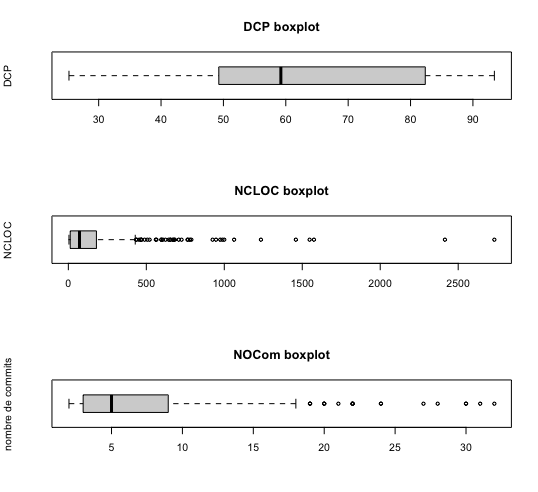
\includegraphics[width=8cm]{boxplot.png} }}%
    \qquad
    \subfloat{{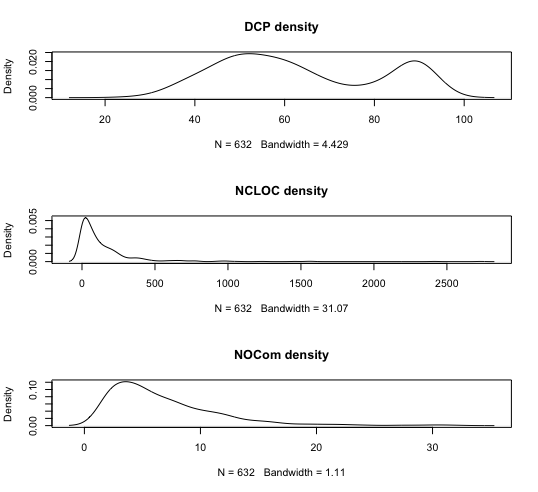
\includegraphics[width=8cm]{density.png} }}%
    \label{fig:example}%
    
    \begin{flushleft}
    Métrique analysis:\\
    \centering
        \subfloat{{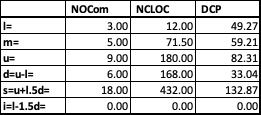
\includegraphics[width=8cm]{images/T1-stats.png} }}%
    \end{flushleft}
    \begin{flushleft}
    NOCom:\\
    On peut voir qu'il y a beaucoup de points en-dehors du limite supérieure dans le diagramme de boîte (Point extrdême). La "queue" est sur le côté droit de la distribution.Donc 
    la distribution est asymétrique à droite.\\
    
    DCP:\\
    Il n'y a pas de point extrdême dans la distributionde DCP. Mais la distribution de DCP n'est pas normalement distributé
    \\
    
    NCLOC:\\
    On peut aussi voir qu'il y a beaucoup de points en-dehors du limite supérieure dans le diagramme de boîte (Point extrdême) pour NCLOC. La "queue" est sur le côté droit de la distribution.Donc 
    la distribution est asymétrique à droite.\\
    \end{flushleft}
}




\section*{Tâche 2}
\answer{
\centering
\subfloa{{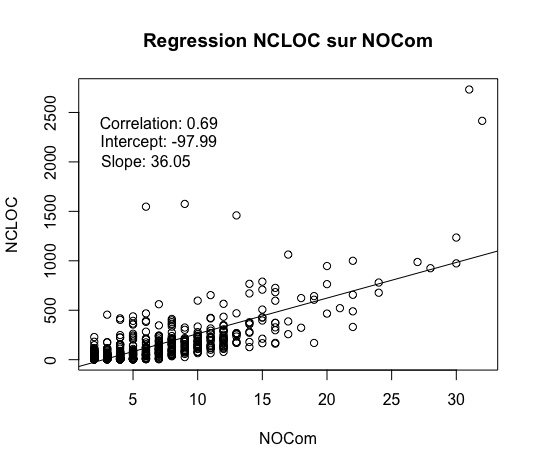
\includegraphics[width=8cm]{images/Rplot-NCLOC-NOCom.png} }}%
\qquad
\subfloat{{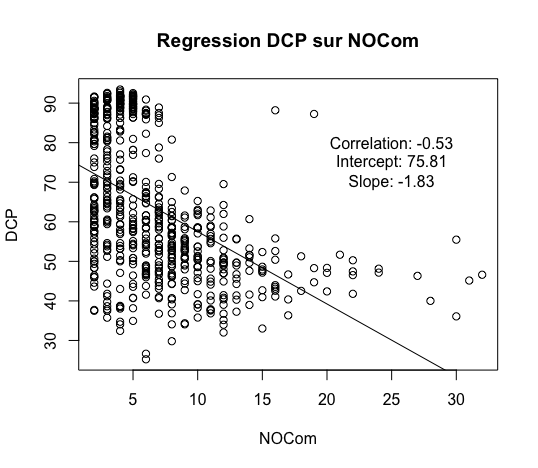
\includegraphics[width=8cm]{images/Rplot-NOCom-DCP.png} }}%
\subfloa{{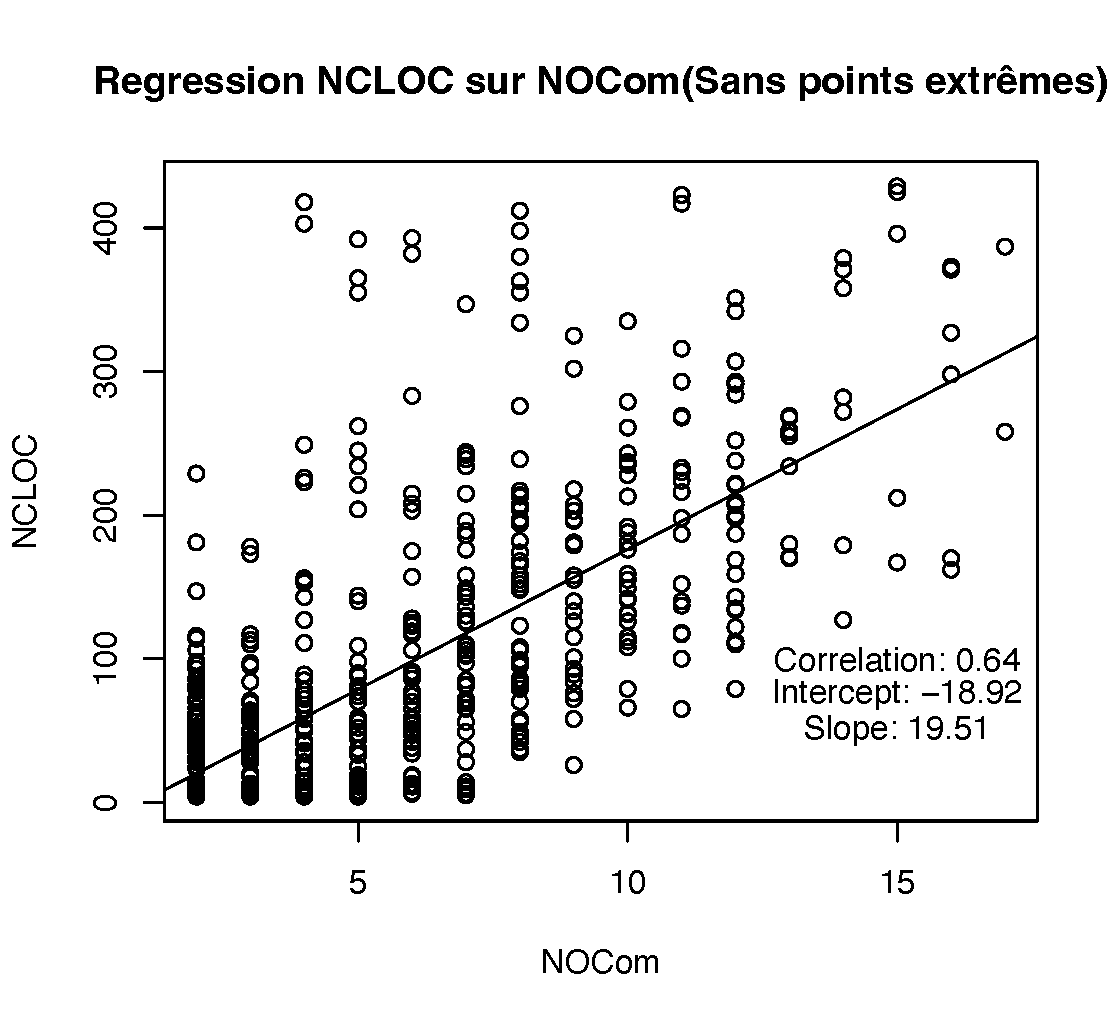
\includegraphics[width=8cm]{images/Rplot01.png} }}%
\qquad
\subfloat{{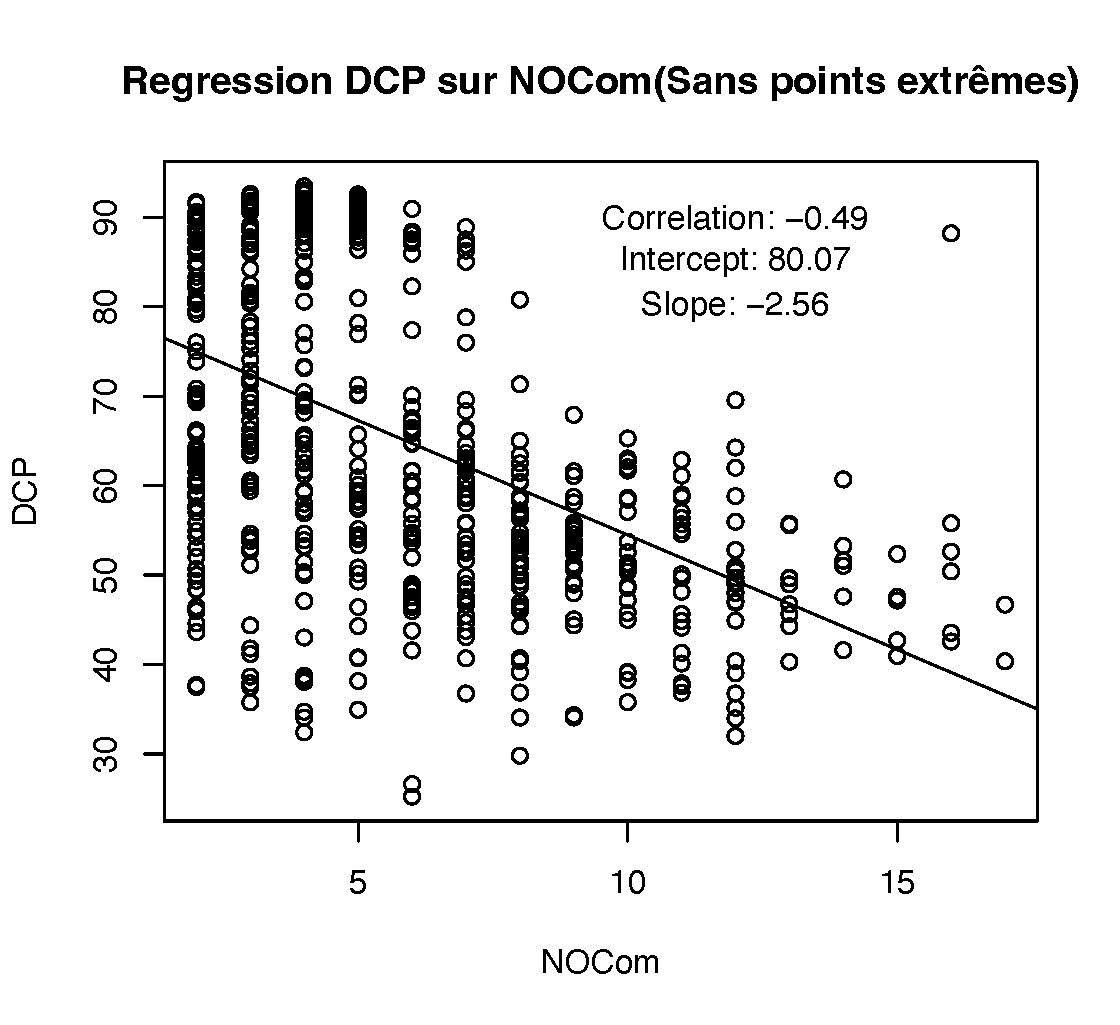
\includegraphics[width=8cm]{images/Rplot02.png} }}%
\label{fig:example}%
    
\begin{flushleft}
(1) Corrélation:\\
Comme les variables NCLOC,DCP et NOCom ne sont pas normalement distribué, il faut utiliser "spearman" pour calculer les correlations entre eux. nous avons:\\
Corr(NOCom,NCLOC)=0.69;Corr(NOCom,NCLOC)=0.64(Sans points extrêmes)\\
La corrélation entre NOCom et NCLOC est positive et plus que 0.6,On peut dire que NOCom et NCLOC sont positivement corrélés.\\
Corr(NOCom,DCP)=-0.53;Corr(NOCom,DCP)=-0.49(Sans points extrêmes)\\
La corrélation entre NOCom et DCP est négative,c'est pas loin de -0.6, on peut dire que NOCom et DCP sont négativement corrélés.\\

(2) Regression:\\
    Modèle de regression:y=a+bx\\
On prend variable NOCom comme variable indépendante(x) et NCLOC comme variable de dépendante(y), on fait la regression, on a a=-97.99,b=36.05/a=-18.92,b=19.51(Sans points extrêmes). b est la pente de la regression qui est positive. c'est à dire que les classes qui ont été modificées plus ont NOCLOC plus élevé. Ceci correspond aux corrélation entre NCLOC et NOCom.\\
On prend variable NOCom comme variable indépendante(x) et DCP comme variable de dépendante(y), on fait la regression, on a a=75.81,b=-1.83/a=80.07,b=-2.56(Sans points extrêmes). b est la pente de la regression qui est négative.c'est à dire que les classes qui ont été modificées plus ont DCP moins élevé. ceci correspond aux corrélation entre DCP et NOCom.\\
\end{flushleft}
}


\section*{Tâche 3}
\answer{
1. Choix d'étude:\\
Quasi-expériance \\
Justification : \\
i) Nécessité de refléter la relation de cause à effet entre les variables indépendantes et dépendantes. Selon l'hypothèse "les classes qui ont été modifiées plus de 10 fois sont mieux commentées que celles qui ont été modifiées moins de 10 fois", nous devons refléter la relation selon laquelle plus le nombre de modifications est élevé, mieux c'est commenté.\\
ii) Affectation aux groupes contrôlée. Nous devons diviser les données de test en deux groupes de manière non aléatoire (classes modifiées plus de dix fois et classes modifiées moins de dix fois).\\
\\
2. Enoncé des hypothèses:
les classes qui ont été modifiées plus de 10 fois sont mieux commentées que celles qui ont été modifiées moins de 10 fois\\
Evaluez l'hypothèse: $H_0$: il n'y a pas de différence entre les classes qui ont été modifiées plus de 10 fois et qui ont été modifiées moins de 10 fois \\
\\
3. Définition des variables:\\
Variables indépendantes: NoCom\\
Variables dépendantes: DCP\\
On utilise le DCP pour mesurer le niveux de commentaire entre des classes.On aussi utilse le NoCom pour diviser des donnée en deux groupes.Un group dont les classes ont été modifiées plus de 10 foid.Un group dont les classes ont été modifiées équal ou moins de 10 fois.Le raison qu'on n'a pas choisi NCLOC comme variable c'est que NCLOC mesure pas le niveau de commentaires.\\
\\
4. Interprétation et généralisation des résultats:\\
\begin{center}
    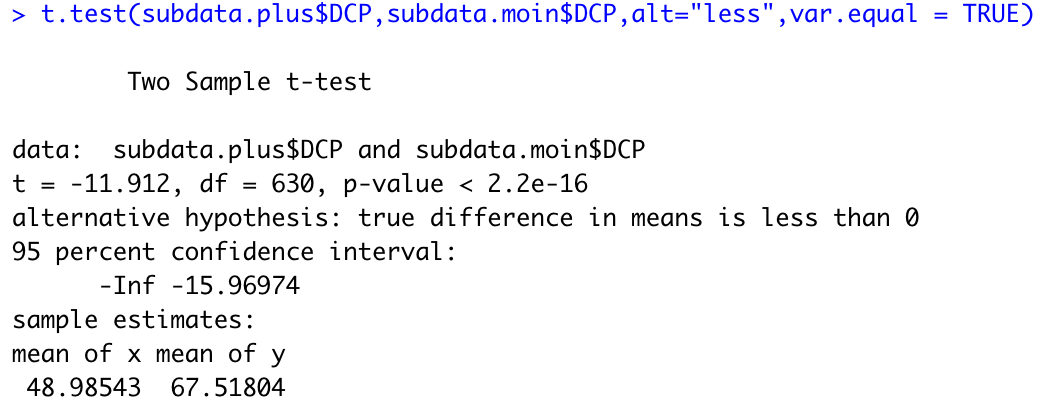
\includegraphics[width=1\columnwidth]{T3.png}
\end{center}
Nous supposons ici que plus la valeur DCP est élevée, la classe est plus mieux commentée.\\
p-value est inférieure à 0,05, on rejete l'hypothèses initial "il n'y a pas de différence entre les classes qui ont été modifiées plus de 10 fois et qui ont été modifiées moins de 10 fois". On accepte l'hypothèses "Le DCP d'une classe modifiée plus de 10 fois est plus petit que le DCP d'une classe modifiée moins de 10 fois." Alors, autrement dit, les classes qui ont été modifiées plus de 10 fois sont moins bien commentées que celles qui ont été modifiées moins de 10 fois.\\
\\
5. Menaces à la validité:\\
Validité de construction: Définir le résultat prévu de manière trop restrictive. La définition du "mieux commenté" est trop restrictive en termes de densité des commentaires(DCP). Le "mieux commenté" est défini de manière plus large.\\
Validité interne: Instrumentalité. Comme les données ne sont pas normalement distribuées, les résultats obtenus à partir du test utilisant le T-Test peuvent ne pas être exacts.\\
% Validité externe: \\
Validité de conclusion: Tous les menaces à la validité interne.\\
}
\end{document}
